\section{Statistical analysis} 

\subsection{a)}
The variables included in the data set are: Id, BMI, age and fast food; all of them are quantitative and they represent:
\begin{itemize}
    \item Id : the respondent's id number 
    \item BMI: respondent's body mass index in $(kg/m^2)$
    \item Age: Respondent's age (in years)
    \item Fast food: fast food consumption per year
\end{itemize}
The total observations are 847, with 3 different variables, so 847 observations for every variable. \\
Here is presented a table containing summary statistics:
\begin{table}[h!]
\centering
\begin{tabular}{|c||c|c|c|c|c|c|c|}
  \hline
\parbox{1.5cm}{\textbf{Variable}} & \textbf{N. of obs.} & \parbox{1.5cm}{\textbf{Sample mean}} & \parbox{1.5cm}{\textbf{Sample std. dev.}} & \parbox{1.5cm}{\textbf{Lower quart.}} & \textbf{Median} & \parbox{1.5cm}{\textbf{Upper quart}} \\ 
 \hline
  & $n$ & $(\overline{x})$ & $(s^2)$ & $(Q_1)$ & $(Q_2)$ & $(Q_3)$ \\
  \hline
  \hline
BMI & 847 & 25.57 & 4.22 & 22.64 & 24.93 & 28.04 \\ 
  \hline
Log-BMI & 847 & 3.23 & 0.16 & 3.12 & 3.22 & 3.33 \\ 
    \hline
Age & 847 & 44.62 & 14.53 & 32.00 & 44.00 & 57.00 \\ 
   \hline
Fast food & 847 & 19.04 & 32.65 & 6.00 & 6.00 & 24.00 \\ 
   \hline
\end{tabular}
\caption{Summary of variables}
\label{SumAll}
\end{table} 
\newpage
Analysis of Log-BMI values: \\
In figure \ref{HistLog} we can observe a histogram representing the empirical density. From here it is easy to tell that the empirical distribution is almost symmetrical and only tends to be slightly right-skewed. The majority of people have a Log-BMI that lies in between 3.1 and 3.3, while there is a big range of variation since some values go from 2.85 (severely underweight) to 3.7 (stage 2 obesity). Looking at figure \ref{BoxLog} we can see the box plot for these values. It helps us to point out where the quantiles, the median and the outliers are located in the distribution. It is almost possible to say that the distribution is symmetrical (only slightly skewed); but surely it can become symmetrical not considering the two or three outliers. \\ 
\begin{figure}[ht!]
\centering
\begin{minipage}{.5\textwidth}
  \centering
  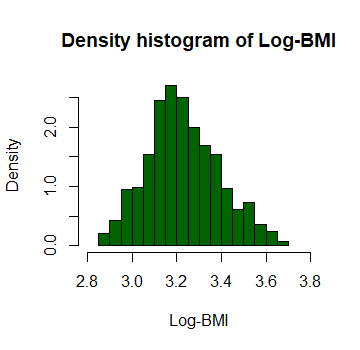
\includegraphics[width=1\linewidth]{root/Hist_log.png}
  \captionof{figure}{Histogram for Log-BMI}
  \label{HistLog}
\end{minipage}%
\begin{minipage}{.5\textwidth}
  \centering
  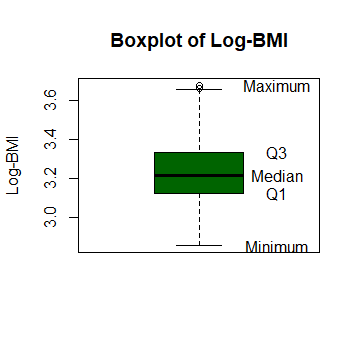
\includegraphics[width=1\linewidth]{root/Box_log.png}
  \captionof{figure}{Boxplot for Log-BMI}
  \label{BoxLog}
\end{minipage}
\end{figure}
\newpage
Analysis of age values: \\
In figure \ref{HistAge} we can observe a histogram representing the empirical density. From here it is easy to tell that the empirical distribution is symmetrical. The majority of people have an age that lies in the range 23-25, 48-50 and 55-57 while there the range of variation goes from 15 to 75. Looking at figure \ref{BoxAge} we can see the box plot for these values. It helps us to point out where the quantiles, the median and the outliers are located in the distribution. Even from here we can confirm that the distribution is symmetrical with no outliers. \\
\begin{figure}[ht!]
\centering
\begin{minipage}{.5\textwidth}
  \centering
  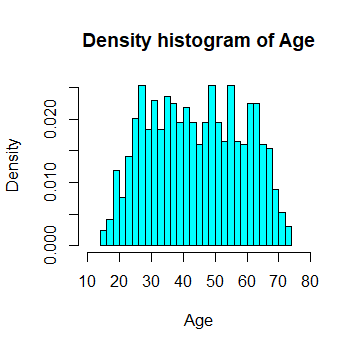
\includegraphics[width=1\linewidth]{root/Hist_age.png}
  \captionof{figure}{Histogram for age}
  \label{HistAge}
\end{minipage}%
\begin{minipage}{.5\textwidth}
  \centering
  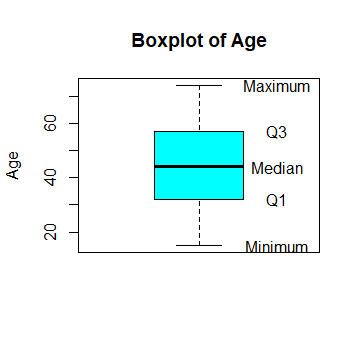
\includegraphics[width=1\linewidth]{root/Box_age.png}
  \captionof{figure}{Boxplot for age}
  \label{BoxAge}
\end{minipage}
\end{figure}
\newpage
Analysis of fast food consumption values: \\
In figure \ref{HistFast} we can observe a histogram representing the empirical density. From here it is easy to tell that the empirical distribution is not symmetrical at all. The majority of people eat fast food a few times a year while there are some that identify as outliers. Looking at figure \ref{BoxFast} we can see the box plot for these values. It does not helps us to point out where the quantiles, the median and the outliers are located in the distribution because is not a proper distribution, in fact from it we can only notice the multiple outliers. \\ 
\begin{figure}[ht!]
\centering
\begin{minipage}{.5\textwidth}
  \centering
  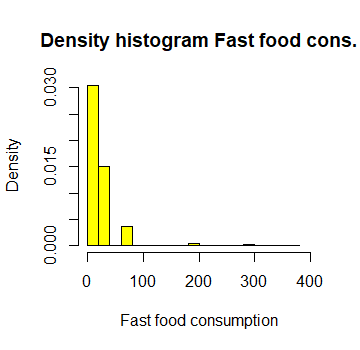
\includegraphics[width=1\linewidth]{root/Hist_fast.png}
  \captionof{figure}{Histogram for fast food cons.}
  \label{HistFast}
\end{minipage}%
\begin{minipage}{.5\textwidth}
  \centering
  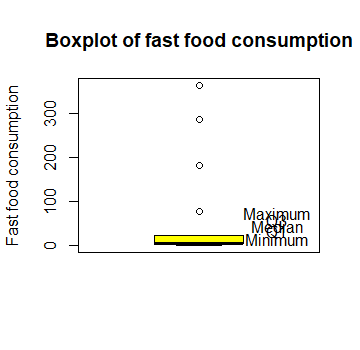
\includegraphics[width=1\linewidth]{root/Box_fast.png}
  \captionof{figure}{Boxplot for fast food cons.}
  \label{BoxFast}
\end{minipage}
\end{figure}
\newpage
Using the scatterplots in figure \ref{ScatLogAge} and \ref{ScatLogFast} it is possible to see if there is correlation between the Log-BMI and the other two variables. Unfortunately in both case the correlation is non existent or really small (might be the case of figure \ref{ScatLogAge}). \\
\begin{figure}[ht!]
\centering
\begin{minipage}{.5\textwidth}
  \centering
  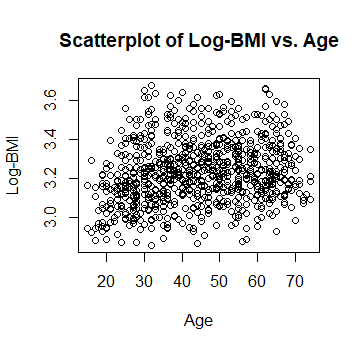
\includegraphics[width=1\linewidth]{root/Scat_log_age.png}
  \captionof{figure}{Scatterplot of Log-BMI vs. age}
  \label{ScatLogAge}
\end{minipage}%
\begin{minipage}{.5\textwidth}
  \centering
  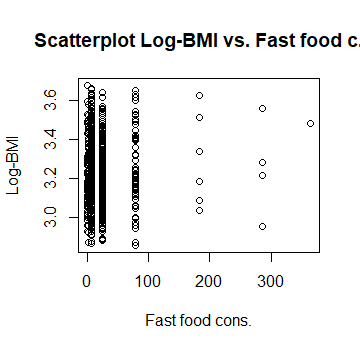
\includegraphics[width=1\linewidth]{root/Scat_log_fast.png}
  \captionof{figure}{Scatterplot Log-BMI vs fast food c.}
  \label{ScatLogFast}
\end{minipage}
\end{figure}

\subsection{b)}
In order to create a multiple linear regression model (MLR)
we set $Y_i$, the Log-BMI scores, as the dependent variable, $x_1$, age and $x_2$ fast food consumption as the independent variables. We also have that $\beta_0$ will be the intercept with the y-axis, $\beta_1$ and $\beta_2$ will the slope for $x_1$ and $x_2$. In conclusion $\epsilon_i$ will be the residual with an unknown variance and a mean of zero. With these assumptions the model can be set up in the following way:
\[ Y_i=\beta_0 +\beta_1 x_{1,i} + \beta_2 x_{2,i}+ \epsilon_i \; \; \; \; \; \; \epsilon_i \sim N(0,\sigma^2)\]

\subsection{c)}
The parameters of the model can be estimated using R. Only the first 840 data points are considered to estimate the parameters (last 7 will be used to validate the parameters). $\hat{\beta_0}$, the intercept is $3.1124$ with a standard deviation of $0.0193$. $\hat{\beta_1}$ which is the slope of the age variable ($x_1$) has a value of $0.0024$, with a standard deviation of $0.0004$. $\hat{\beta_2}$ which is the slope of fast food consumption variable ($x_2$) has a value of $0.0005$ and a standard deviation of $0.0002$. it can be noticed that $\hat{\beta_1}$ and $\hat{\beta_2}$ increase slowly since their values are close to 0 but still positive. We can find the degrees of freedom used in all the calculations with the following formula: 
\begin{equation}\label{dof}
    DF=n-(p+1)=840-(2+1)=837
\end{equation}
The variance of the residuals is $\hat{\sigma}^2=0.1573^2$ and the explained variation $R^2=0.0449^2$.

\subsection{d)}
For every model that is set up we must check if it is valid. To do so we are going to use multiple plots in order asses our validation. \\
\begin{figure}[!h]
  \centering
  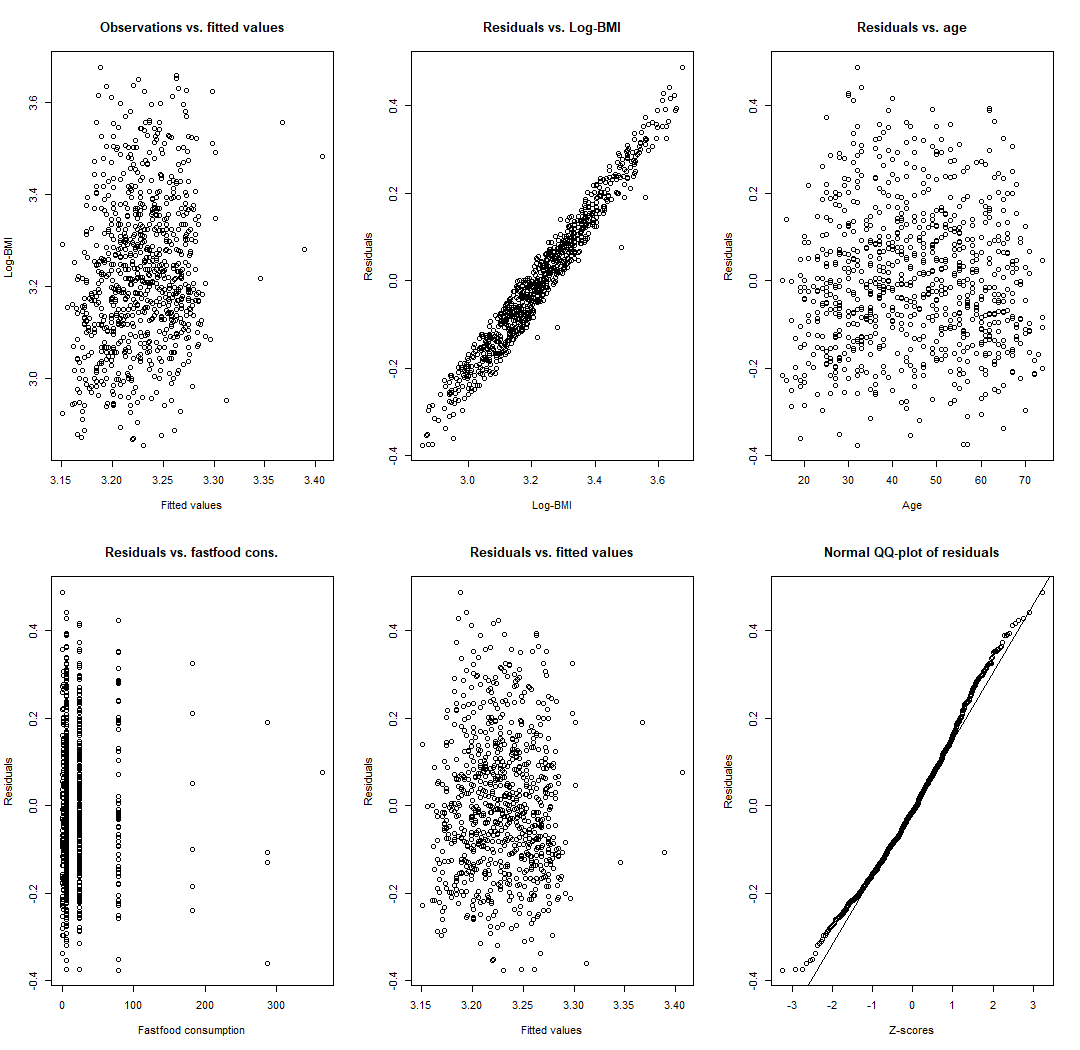
\includegraphics[width=0.75\linewidth]{root/Model_val.png}
  \captionof{figure}{Plots for model validation}
  \label{ModelVal}
\end{figure} \\
From the plot "Observations against fitted values" we are not able to see any correlation between the data points, this indicates that the data is normally distributed, which is true because of the independence of the observations. This can also be seen on the plot "Residuals against Log-BMI", where the data points form a straight line, that indicates a linear relationship between the fitted values and Log-BMI. For the graphs "Residuals against age" and "Residuals against fast food consumption" we can see that that there is no correlation between the variables and their residuals. This is also the case for the plot "Residuals against fitted values" where we can't see any correlation between the residuals. This again suggests that the residuals are independent values, which indicates that the data set is normally distributed. In conclusion we look at the "Normal QQ plot of the residuals", this plot has already been validated in R with the Wallyplot method. Since we were not able to point out our residuals plot, we can be sure that our values are normally distributed. This proves one more time that the observations are independent and normally distributed. The residuals follow a straight line, with few exceptions. This is another hint the suggests that the data set is normally distributed. \\
\begin{figure}[ht!]
  \centering
  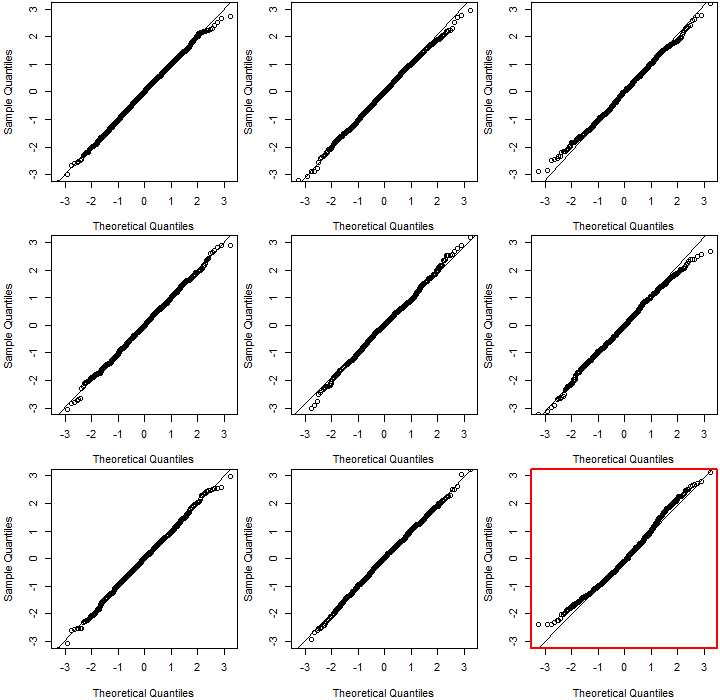
\includegraphics[width=0.75\linewidth]{root/Wally_res.png}
  \captionof{figure}{Wally plot for model validation}
  \label{WallyVal}
\end{figure} \\
It is now possible to state the the model has been validated and the prerequisites are met.

\subsection{e)}
The $95\%$ confidence intervals, denoted by $\beta_1$, for the 
age coefficients is found using this formula.
\[ \hat{\beta_1} \pm t_{1-\alpha/2} \cdot \hat{\sigma}_{\beta_1} \]
Notice that the degrees of freedom are given from the previously stated equation \ref{dof}. Inserting the values into the formula we get:
\begin{equation}\label{CIB1}
CI_{\beta_1} = 0.0024 \pm 1.9628 \cdot 0.0004 = [0.0016 , 0.0031]
\end{equation}
For the two others coefficients we have used the same formula as in equation \ref{CIB1}, with other values. The resulting confidence intervals are:
\[ CI_{\beta_0} = [3.0744 , 3.1504] \]
\[ CI_{\beta_2} = [0.0002 , 0.0008] \]

\subsection{f)}
We would like to test whether $\beta_1$ could have the value 0.001. Therefore, the following null hypothesis can be formulated
with a significance level of $\alpha=0.05$:
\[H_0: \beta_1 =0.001\]
\[H_0: \beta_1 \neq 0.001\]
The formula for the t-test is given by: 
\[ t_{obs,\beta_1}=\frac{\hat{\beta_1}-\beta_1}{\hat{\sigma_{\beta_1}}} = \frac{0.0024-0.001}{0.0004}=3.5\]
To compute the p-values we use the following formula. With the p-value we can state if we have evidence against the null hypothesis. We are using $DF=837$ as stated in equation \ref{dof}. Following the formula:
\[p=2P(T>|t_{obs,\beta_1}|) \]
The calculated p-value is:
\[ p=0.0004 \]
Since the calculated p-value for this hypothesis test is less than the set significance level ($\alpha=0.05$), the null hypothesis must be rejected. Therefore, $\beta_1$ cannot have the value 0.001 within the selected significance level. The same conclusion could have been made looking at the confidence intervals found in the equation \ref{CIB1}.

\subsection{g)}
We can reduce our model by using backward selection. This means that we can remove the variables from the model that are not significant. This allows us to simplify our model. However from the R code we can see that the p-values are less than the significance level $\alpha = 0.05$, so they are significant. We could also try to create a new model and see if there are big differences, with R we read:
\[ p_{\beta_1} = 1.58 \cdot 10^{-9}\]
\[ p_{\beta_2} = 1.88 \cdot 10^{-3}\]
From here we could choose to eliminate the fast food consumption from the model and see if the difference is enough to make the change. The p-value and the estimates for the new parameter $\beta_1$ are:
\[ \beta_1 = 0.0020\]
\[ p_{\beta_1} = 8.15 \cdot 10^{-8}\]
From these values we can see that there is a difference but it's not much; therefore  all the variables are significant. This means that the final model is the same as the model that was initially determined and there is no need to do backward selection.

\subsection{h)}
Predictions and $95\%$ prediction intervals for Log-BMI values are determined for each of the seven observations in the data set (D\_test) to be used to validate the final model. The R function "predict" has been used to calculate predictions and the $95\%$ prediction intervals of every value. These can be seen in table \ref{PredAndCI} below:
\begin{table}[h!]
\centering
\begin{tabular}{|c||c|c||c|}
  \hline
ID & Log-BMI & Prediction & CIs \\
 \hline
 \hline
841 & 3.1434 & 3.2370 & [2.9280, 3.5460] \\
\hline
842 & 3.2692 & 3.2109 & [2.9018, 3.5199] \\
\hline
843 & 3.2694 & 3.2322 & [2.9232, 3.5413] \\
\hline
844 & 3.3242 & 3.2322 & [2.9232, 3.5413] \\
\hline
845 & 3.1065 & 3.2299 & [2.9209, 3.5389] \\
\hline
846 & 3.2638 & 3.2296 & [2.9206, 3.5387] \\
\hline
847 & 3.0585 & 3.2117 & [2.9019, 3.5214] \\
\hline
\end{tabular}
\caption{Predictions and confidence intervals for test data}
\label{PredAndCI}
\end{table} 
From the table we can see that both the predictions and the observed Log-BMI lie within the prediction interval for the model. This shows that the model is accurate in relation to the calculation of these values since they fall within the permitted CIs for all observations. We can state that this is an accurate model for the Log-BMI values.